\documentclass[xcolor=svgnames]{beamer}\usepackage[]{graphicx}\usepackage[]{color}
%% maxwidth is the original width if it is less than linewidth
%% otherwise use linewidth (to make sure the graphics do not exceed the margin)
\makeatletter
\def\maxwidth{ %
  \ifdim\Gin@nat@width>\linewidth
    \linewidth
  \else
    \Gin@nat@width
  \fi
}
\makeatother

\definecolor{fgcolor}{rgb}{0.345, 0.345, 0.345}
\newcommand{\hlnum}[1]{\textcolor[rgb]{0.686,0.059,0.569}{#1}}%
\newcommand{\hlstr}[1]{\textcolor[rgb]{0.192,0.494,0.8}{#1}}%
\newcommand{\hlcom}[1]{\textcolor[rgb]{0.678,0.584,0.686}{\textit{#1}}}%
\newcommand{\hlopt}[1]{\textcolor[rgb]{0,0,0}{#1}}%
\newcommand{\hlstd}[1]{\textcolor[rgb]{0.345,0.345,0.345}{#1}}%
\newcommand{\hlkwa}[1]{\textcolor[rgb]{0.161,0.373,0.58}{\textbf{#1}}}%
\newcommand{\hlkwb}[1]{\textcolor[rgb]{0.69,0.353,0.396}{#1}}%
\newcommand{\hlkwc}[1]{\textcolor[rgb]{0.333,0.667,0.333}{#1}}%
\newcommand{\hlkwd}[1]{\textcolor[rgb]{0.737,0.353,0.396}{\textbf{#1}}}%

\usepackage{framed}
\makeatletter
\newenvironment{kframe}{%
 \def\at@end@of@kframe{}%
 \ifinner\ifhmode%
  \def\at@end@of@kframe{\end{minipage}}%
  \begin{minipage}{\columnwidth}%
 \fi\fi%
 \def\FrameCommand##1{\hskip\@totalleftmargin \hskip-\fboxsep
 \colorbox{shadecolor}{##1}\hskip-\fboxsep
     % There is no \\@totalrightmargin, so:
     \hskip-\linewidth \hskip-\@totalleftmargin \hskip\columnwidth}%
 \MakeFramed {\advance\hsize-\width
   \@totalleftmargin\z@ \linewidth\hsize
   \@setminipage}}%
 {\par\unskip\endMakeFramed%
 \at@end@of@kframe}
\makeatother

\definecolor{shadecolor}{rgb}{.97, .97, .97}
\definecolor{messagecolor}{rgb}{0, 0, 0}
\definecolor{warningcolor}{rgb}{1, 0, 1}
\definecolor{errorcolor}{rgb}{1, 0, 0}
\newenvironment{knitrout}{}{} % an empty environment to be redefined in TeX

\usepackage{alltt}
\usetheme{Boadilla}
\usecolortheme[named=SeaGreen]{structure}
\usepackage{graphicx}
\usepackage{breqn}
\usepackage{xcolor}
\usepackage{booktabs}
\usepackage{verbatim}
\usepackage{tikz}
\usepackage{lmodern}
\usetikzlibrary{shadows,arrows,positioning}
\definecolor{links}{HTML}{2A1B81}
\hypersetup{colorlinks,linkcolor=links,urlcolor=links}
\usepackage{pgfpages}

\newcommand{\Bigtxt}[1]{\textbf{\textit{#1}}}
\IfFileExists{upquote.sty}{\usepackage{upquote}}{}
\begin{document}

\title[Exploratory Data Analysis]{Exploratory Data Analysis with SWMP}

\author[M. Beck, T. O'Brien]{Marcus W. Beck\inst{1} \and Todd D. O'Brien\inst{2}}

\date{}

\institute[]{\inst{1} ORISE, USEPA NHEERL Gulf Ecology Division\\ Email: \href{mailto:beck.marcus@epa.gov}{beck.marcus@epa.gov} \and \inst{2} NOAA/NMFS COPEPOD Project\\ Email: \href{todd.obrien@noaa.gov}{todd.obrien@noaa.gov}}

% knitr setup


% load SWMPr from local


%%%%%%
\begin{frame}
\vspace{0.3in}
\centerline{
\begin{tikzpicture}
  \node[drop shadow={shadow xshift=0ex,shadow yshift=0ex},fill=white,draw] at (0,0) {
\includegraphics[width=0.9\textwidth]{bg_main.jpg}};
\end{tikzpicture}}
\titlepage
\end{frame}

%%%%%%
\begin{frame}{Objectives and agenda}
\begin{itemize}
\onslide<+->
\item Objectives \\~\\
\begin{itemize}
\item What are some basic time series analysis techniques and when would you use them? \\~\\
\item How are the data set up, what functions are used, and how are the results interpreted? \\~\\
\end{itemize}
\onslide<+->
\item Agenda \\~\\
\begin{itemize}
\item Analysis 1 - missing data and interpolation\\~\\
\item Analysis 2 - smoothing and aggregation \\~\\
\item Analysis 3 - basic trend analysis\\~\\
\end{itemize}
\end{itemize}
\end{frame}

%%%%%%
\begin{frame}{Interactive portion}
You can follow along in this module: \\~\\
\begin{itemize}
\item dataset3 \\~\\
\item script3 \\~\\
\end{itemize}
\Large
\centerline{\emph{Interactive!}}
\end{frame}

%%%%%%
\begin{frame}{What is exploratory data analysis (EDA)?}
A general term that describes preliminary evaluation of a variable or multiple variables in a dataset to assess quantitative properties for further analysis or hypothesis generation\\~\\
EDA can inform you of the \alert{types} of variables (categorical, continuous), \alert{distribution} of variables (central tendency, spread), \alert{correlations} between variables, and presence of \alert{outliers} \\~\\
R has many functions available for EDA - see the \href{http://cran.r-project.org/doc/contrib/Short-refcard.pdf}{R reference card} and the cookbook for some ideas\\~\\
For now, we will focus on some tasks that have specific relevance to SWMP
\end{frame}

%%%%%%
\begin{frame}[containsverbatim]{Analysis 1 - Missing data and interpolation}
Time series will usually include missing data - you will have to decide how to handle missing values \\~\\
Let's import some wq data

\begin{knitrout}\scriptsize
\definecolor{shadecolor}{rgb}{0.969, 0.969, 0.969}\color{fgcolor}\begin{kframe}
\begin{alltt}
\hlcom{# import data, qaqc, and subset}
\hlcom{# change this path for the flash drive}
\hlstd{path} \hlkwb{<-} \hlstr{'C:/data/dataset3'}
\hlstd{dat} \hlkwb{<-} \hlkwd{import_local}\hlstd{(path,} \hlstr{'cbmmcwq2012'}\hlstd{)}
\end{alltt}
\end{kframe}
\end{knitrout}
\begin{knitrout}\scriptsize
\definecolor{shadecolor}{rgb}{0.969, 0.969, 0.969}\color{fgcolor}\begin{kframe}
\begin{alltt}
\hlcom{# qaqc and subset do_mgl}
\hlstd{dat} \hlkwb{<-} \hlkwd{qaqc}\hlstd{(dat)}
\hlstd{dat} \hlkwb{<-} \hlkwd{subset}\hlstd{(dat,} \hlkwc{select} \hlstd{=} \hlstr{'do_mgl'}\hlstd{)}

\hlcom{# how many missing values?}
\hlkwd{sum}\hlstd{(}\hlkwd{is.na}\hlstd{(dat}\hlopt{$}\hlstd{do_mgl))}
\end{alltt}
\begin{verbatim}
## [1] 419
\end{verbatim}
\end{kframe}
\end{knitrout}
\end{frame}

%%%%%%
\begin{frame}[containsverbatim]{Analysis 1 - Missing data and interpolation}
Introducing the `na.approx' function - this method can interpolate missing data
\begin{knitrout}\scriptsize
\definecolor{shadecolor}{rgb}{0.969, 0.969, 0.969}\color{fgcolor}\begin{kframe}
\begin{alltt}
\hlcom{# subset the do time series for plotting}
\hlstd{wq_dat} \hlkwb{<-} \hlkwd{subset}\hlstd{(wq_dat,} \hlkwc{subset} \hlstd{=} \hlkwd{c}\hlstd{(}\hlstr{'2012-10-01 0:0'}\hlstd{,} \hlstr{'2012-10-31 0:0'}\hlstd{))}
\hlkwd{plot}\hlstd{(do_mgl} \hlopt{~} \hlstd{datetimestamp, wq_dat,} \hlkwc{type} \hlstd{=} \hlstr{'l'}\hlstd{)}
\end{alltt}
\end{kframe}

{\centering 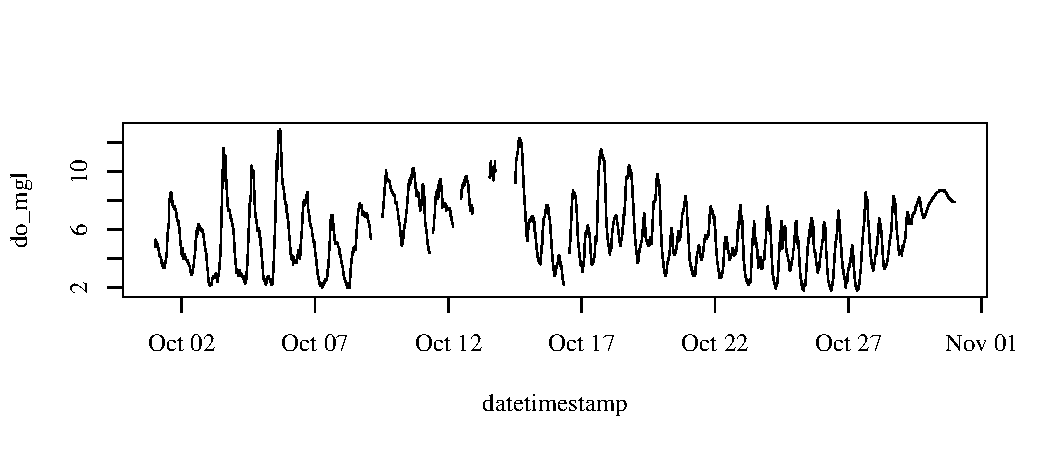
\includegraphics[width=0.8\textwidth]{figure/unnamed-chunk-4} 

}



\end{knitrout}
Notice the missing values around October 12\textsuperscript{th}
\end{frame}

%%%%%%
\begin{frame}[containsverbatim]{Analysis 1 - Missing data and interpolation}
Here's what the time series looks like after using `na.approx'
\begin{knitrout}\scriptsize
\definecolor{shadecolor}{rgb}{0.969, 0.969, 0.969}\color{fgcolor}

{\centering 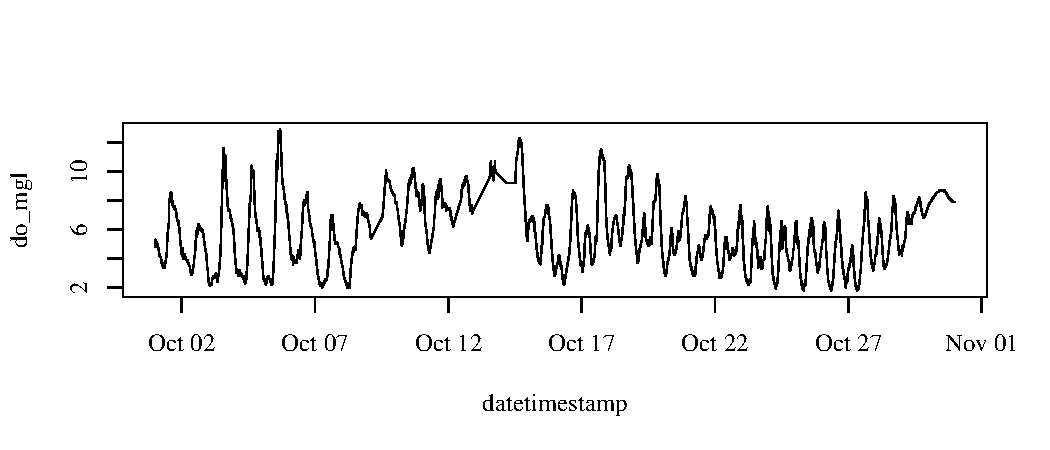
\includegraphics[width=0.8\textwidth]{figure/unnamed-chunk-5} 

}



\end{knitrout}
The missing values have been linearly interpolated - a simple function that predicts missing values based on the starting and ending values in gaps
\end{frame}

%%%%%%
\begin{frame}[containsverbatim]{Analysis 1 - Missing data and interpolation}
The `na.approx.swmpr' function has only a few arguments\\~\\
\begin{itemize}
\item object: input swmpr data \\~\\
\item params: which parameters to interpolate, default is all \\~\\
\item maxgap: what is the maximum gap size to interpolate (units are the timestep)?
\end{itemize}
See the help file for moreinfo
\begin{knitrout}\scriptsize
\definecolor{shadecolor}{rgb}{0.969, 0.969, 0.969}\color{fgcolor}\begin{kframe}
\begin{alltt}
\hlcom{# see the help file}
\hlopt{?}\hlstd{na.approx.swmpr}
\end{alltt}
\end{kframe}
\end{knitrout}
\end{frame}

%%%%%%
\begin{frame}[containsverbatim]{Analysis 1 - Missing data and interpolation}
Now you try an analysis! Open a new script and try the following: \\~\\
\begin{itemize}
\item Import the file `cbmmcwq2012.csv' in the dataset3 folder \\~\\
\item Handle QAQC flags and subset by October 1 to 31 \\~\\
\item Plot the data - where are the missing values?\\~\\
\item Use `na.approx.swmpr' to interpolate the missing values - what value to use for maxgap?\\~\\
\item Plot the data again - how does it look?
\end{itemize}
\end{frame}

%%%%%%
\begin{frame}[containsverbatim]{Analysis 2 - Smoothing and aggregation}
\alert{Problem}: trend evaluation is difficult if the data are noisy \\~\\
Noise can be addressed by\alert{aggregating} or \alert{smoothing} data, both are similar \\~\\
The \alert{`aggregate.swmpr'} function aggregates a time series by set periods of observation and calculates summary data for a parameter(s) \\~\\
The \alert{`smoother.swmpr'} function calculates a moving window average of a time series \\~\\
\end{frame}

%%%%%%
\begin{frame}[containsverbatim]{Analysis 2 - Smoothing and aggregation}
The (relevant) arguments for `aggregate.swmpr':\\~\\
\begin{itemize}
\item x: Input data object \\~\\
\item by: How are the data aggregated - `years', `quarters', `months', `weeks', `days', `hours' \\~\\
\item FUN: What function is used to aggregate the data? Defaults to mean.\\~\\
\item aggs\_out: T or F, to return the data at an intermediate step for plotting
\end{itemize}
\begin{knitrout}\scriptsize
\definecolor{shadecolor}{rgb}{0.969, 0.969, 0.969}\color{fgcolor}\begin{kframe}
\begin{alltt}
\hlcom{# see help for all arguments}
\hlopt{?}\hlstd{aggregate.swmpr}
\end{alltt}
\end{kframe}
\end{knitrout}
\end{frame}

%%%%%%
\begin{frame}[containsverbatim]{Analysis 2 - Smoothing and aggregation}
The (relevant) arguments for `smoother.swmpr':\\~\\
\begin{itemize}
\item swmpr\_in: Input data object \\~\\
\item window: the size of the smoothing window, defaults to five observations at the current time step \\~\\
\item sides: what defines the window, centered on an observation (2, default) or use only the preceding observations (1)  \\~\\
\end{itemize}
\begin{knitrout}\scriptsize
\definecolor{shadecolor}{rgb}{0.969, 0.969, 0.969}\color{fgcolor}\begin{kframe}
\begin{alltt}
\hlcom{# see help for all arguments}
\hlopt{?}\hlstd{smoother.swmpr}
\end{alltt}
\end{kframe}
\end{knitrout}
\end{frame}

%%%%%%
\begin{frame}[containsverbatim]{Analysis 2 - Smoothing and aggregation}
Now you try an analysis! Open a new script and try the following: \\~\\
\begin{itemize}
\item Import the the same data as before - `cbmmcwq2012.csv' in the dataset3 folder \\~\\
\item Handle QAQC flags and subset by October 1 to 31 \\~\\
\item Plot the raw data \\~\\
\item Use `smoother.swmpr', save to new object, plot again. How does it look? Try different window sizes.\\~\\
\item Aggregate the data by weeks and view the raw data (do not plot).  Now try aggregation by months, what's the difference?\\~\\
\end{itemize}
\end{frame}

%%%%%%
\begin{frame}[containsverbatim]{Analysis 2 - Smoothing and aggregation}
\begin{knitrout}\scriptsize
\definecolor{shadecolor}{rgb}{0.969, 0.969, 0.969}\color{fgcolor}\begin{kframe}
\begin{alltt}
\hlcom{# use the same data as in analysis 1 but...}
\hlcom{# subset by these date ranges}
\hlstd{dat} \hlkwb{<-} \hlkwd{subset}\hlstd{(dat,} \hlkwc{subset} \hlstd{=} \hlkwd{c}\hlstd{(}\hlstr{'2012-10-01 0:0'}\hlstd{,} \hlstr{'2012-10-31 0:0'}\hlstd{))}

\hlcom{# smooth }
\hlstd{new_dat} \hlkwb{<-} \hlkwd{smoother.swmpr}\hlstd{(dat,} \hlkwc{window} \hlstd{=} \hlnum{40}\hlstd{)}

\hlcom{# plot original, then new}
\hlkwd{plot}\hlstd{(do_mgl} \hlopt{~} \hlstd{datetimestamp,} \hlkwc{data} \hlstd{= dat,} \hlkwc{type} \hlstd{=} \hlstr{'l'}\hlstd{)}
\hlkwd{plot}\hlstd{(do_mgl} \hlopt{~} \hlstd{datetimestamp,} \hlkwc{data} \hlstd{= new_dat,} \hlkwc{type} \hlstd{=} \hlstr{'l'}\hlstd{)}
\end{alltt}
\end{kframe}
\end{knitrout}
\begin{knitrout}\scriptsize
\definecolor{shadecolor}{rgb}{0.969, 0.969, 0.969}\color{fgcolor}

{\centering 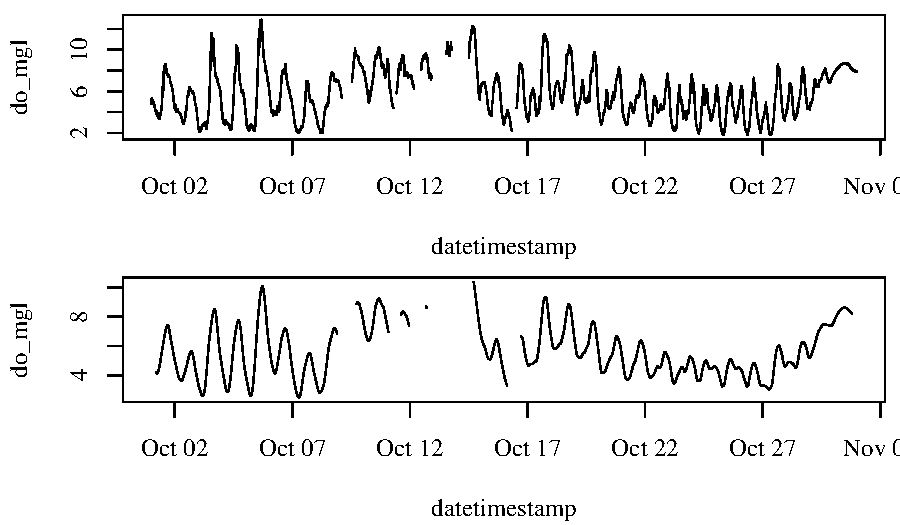
\includegraphics[width=0.7\textwidth]{figure/unnamed-chunk-10} 

}



\end{knitrout}
\end{frame}

%%%%%%
\begin{frame}[containsverbatim]{Analysis 2 - Smoothing and aggregation}
\begin{knitrout}\scriptsize
\definecolor{shadecolor}{rgb}{0.969, 0.969, 0.969}\color{fgcolor}\begin{kframe}
\begin{alltt}
\hlcom{# try an aggregation by 'weeks'}
\hlkwd{aggregate}\hlstd{(dat,} \hlkwc{by} \hlstd{=} \hlstr{'weeks'}\hlstd{)}
\end{alltt}
\begin{verbatim}
##   datetimestamp do_mgl
## 1    2012-09-30    5.4
## 2    2012-10-07    6.4
## 3    2012-10-14    6.6
## 4    2012-10-21    4.5
## 5    2012-10-28    6.2
\end{verbatim}
\begin{alltt}
\hlcom{# try an aggregation by 'months'}
\hlkwd{aggregate}\hlstd{(dat,} \hlkwc{by} \hlstd{=} \hlstr{'months'}\hlstd{)}
\end{alltt}
\begin{verbatim}
##   datetimestamp do_mgl
## 1    2012-10-01    5.8
\end{verbatim}
\end{kframe}
\end{knitrout}
\end{frame}

%%%%%%
\begin{frame}[containsverbatim]{Analysis 3 - Basic trend analysis}
More often, we are concerned with \alert{long-term trends} over time -- a missing data point here or there or noisy data on short time periods may not be very important \\~\\
We need \alert{plots} to characterize long-term trends over time -- both \alert{raw} and \alert{summarized} data \\~\\
This analysis will show you two ways to evaluate trends by plotting
\end{frame}

%%%%%%
\begin{frame}[containsverbatim]{Analysis 3 - Basic trend analysis}
Start by importing all the water quality data for the `Iron Pot Landing' station at the Chesapeake Bay Maryland reserve 

\begin{knitrout}\scriptsize
\definecolor{shadecolor}{rgb}{0.969, 0.969, 0.969}\color{fgcolor}\begin{kframe}
\begin{alltt}
\hlcom{# import all wq data for cbmip}
\hlcom{# change path as needed}
\hlstd{path} \hlkwb{<-} \hlstr{'C:/data/dataset3/'}
\hlstd{dat} \hlkwb{<-} \hlkwd{import_local}\hlstd{(path,} \hlstr{'cbmipwq'}\hlstd{)}

\hlcom{# qaqc checks}
\hlstd{dat} \hlkwb{<-} \hlkwd{qaqc}\hlstd{(dat)}
\end{alltt}
\end{kframe}
\end{knitrout}
\alert{Our questions}: What are the dissolved oxygen dynamics over the last four years?  Can we characterize trends, both seasonal and annual?
\end{frame}

%%%%%%
\begin{frame}[containsverbatim]{Analysis 3 - Basic trend analysis}
First a simple plot...
\begin{knitrout}\scriptsize
\definecolor{shadecolor}{rgb}{0.969, 0.969, 0.969}\color{fgcolor}\begin{kframe}
\begin{alltt}
\hlcom{# plot DO for the time series}
\hlkwd{plot}\hlstd{(do_mgl} \hlopt{~} \hlstd{datetimestamp,} \hlkwc{data} \hlstd{= dat,} \hlkwc{type} \hlstd{=} \hlstr{'l'}\hlstd{)}
\end{alltt}
\end{kframe}

{\centering 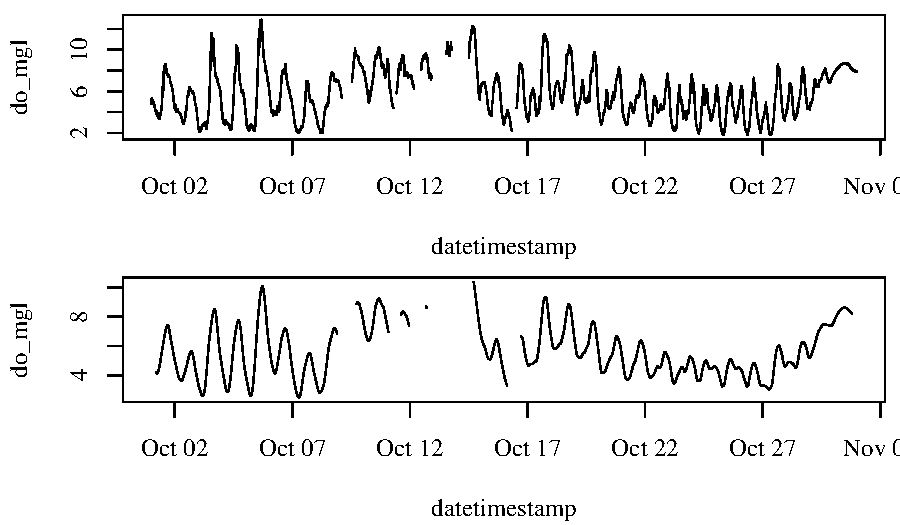
\includegraphics[width=\textwidth]{figure/unnamed-chunk-14} 

}



\end{knitrout}
\end{frame}

%%%%%%
\begin{frame}[containsverbatim]{Analysis 3 - Basic trend analysis}
If we are concerned with long-term trends, we want to reduce the noise related to annual variability...  we can use the smoother function
\begin{knitrout}\scriptsize
\definecolor{shadecolor}{rgb}{0.969, 0.969, 0.969}\color{fgcolor}\begin{kframe}
\begin{alltt}
\hlcom{# smoother using a large window (5000 steps ~ 52 days)}
\hlstd{do_smooth} \hlkwb{<-} \hlkwd{smoother}\hlstd{(dat,} \hlkwc{params} \hlstd{=} \hlstr{'do_mgl'}\hlstd{,} \hlkwc{window} \hlstd{=} \hlnum{5000}\hlstd{)}
\hlkwd{plot}\hlstd{(do_mgl} \hlopt{~} \hlstd{datetimestamp,} \hlkwc{data} \hlstd{= dat,} \hlkwc{type} \hlstd{=} \hlstr{'l'}\hlstd{)}
\hlkwd{lines}\hlstd{(do_smooth}\hlopt{$}\hlstd{datetimestamp, do_smooth}\hlopt{$}\hlstd{do_mgl,} \hlkwc{col} \hlstd{=} \hlstr{'red'}\hlstd{,} \hlkwc{lwd} \hlstd{=} \hlnum{2}\hlstd{)}
\end{alltt}
\end{kframe}

{\centering 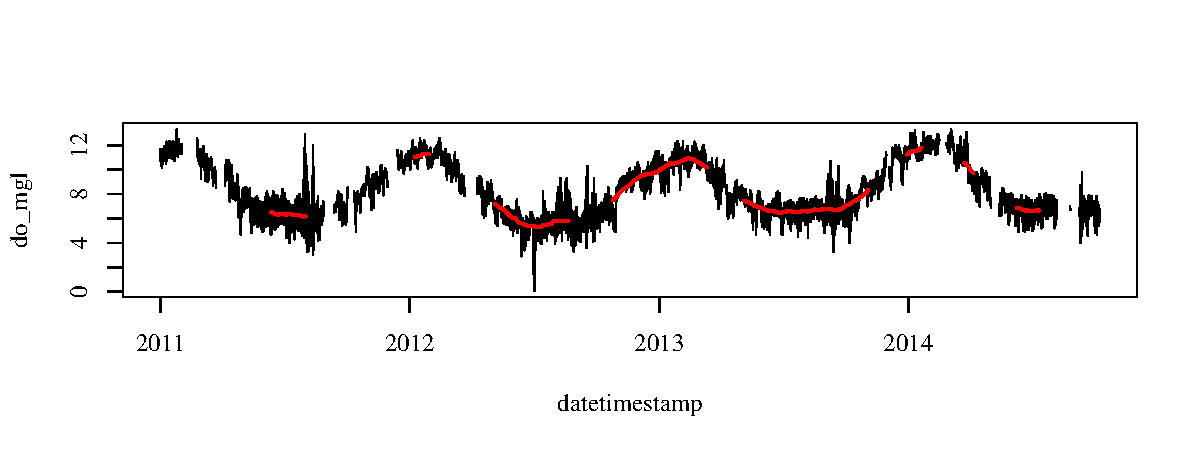
\includegraphics[width=\textwidth]{figure/unnamed-chunk-15} 

}



\end{knitrout}
\end{frame}

%%%%%%
\begin{frame}[containsverbatim]{Analysis 3 - Basic trend analysis}
Try it again but use `na.approx' first to fill gaps
\begin{knitrout}\scriptsize
\definecolor{shadecolor}{rgb}{0.969, 0.969, 0.969}\color{fgcolor}\begin{kframe}
\begin{alltt}
\hlcom{# use na.approx, then smooth}
\hlstd{new_dat} \hlkwb{<-} \hlkwd{na.approx}\hlstd{(dat,} \hlkwc{param} \hlstd{=} \hlstr{'do_mgl'}\hlstd{,} \hlkwc{maxgap} \hlstd{=} \hlnum{3000}\hlstd{)}
\hlstd{do_smooth} \hlkwb{<-} \hlkwd{smoother}\hlstd{(new_dat,} \hlkwc{params} \hlstd{=} \hlstr{'do_mgl'}\hlstd{,} \hlkwc{window} \hlstd{=} \hlnum{5000}\hlstd{)}
\hlkwd{plot}\hlstd{(do_mgl} \hlopt{~} \hlstd{datetimestamp,} \hlkwc{data} \hlstd{= new_dat,} \hlkwc{type} \hlstd{=} \hlstr{'l'}\hlstd{)}
\hlkwd{lines}\hlstd{(do_smooth}\hlopt{$}\hlstd{datetimestamp, do_smooth}\hlopt{$}\hlstd{do_mgl,} \hlkwc{col} \hlstd{=} \hlstr{'red'}\hlstd{,} \hlkwc{lwd} \hlstd{=} \hlnum{2}\hlstd{)}
\end{alltt}
\end{kframe}

{\centering 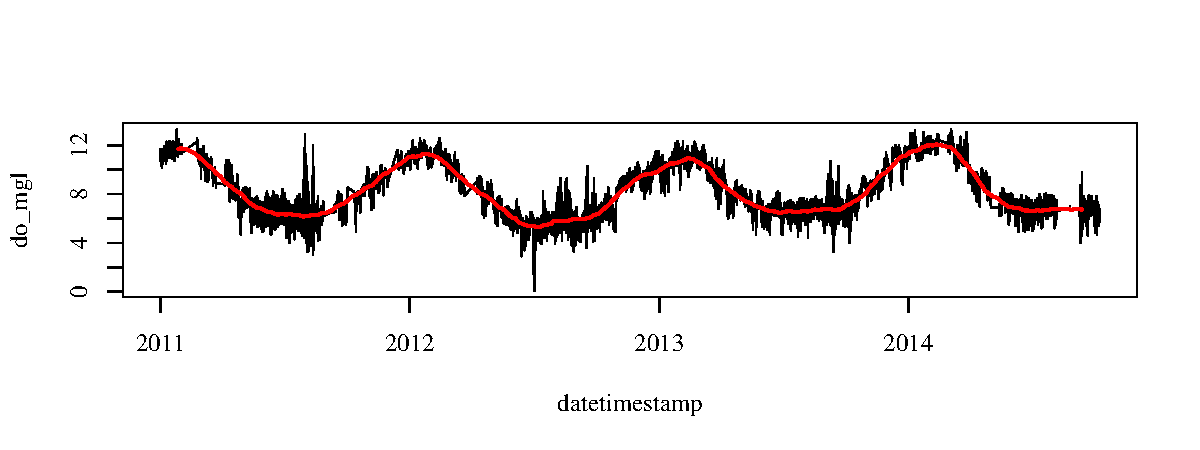
\includegraphics[width=\textwidth]{figure/unnamed-chunk-16} 

}



\end{knitrout}
Now we have a time series that primarily shows annual variation, independent of short-term variation
\end{frame}

%%%%%%
\begin{frame}[containsverbatim]{Analysis 3 - Basic trend analysis}
Finally, we can use the `aggregate.swmpr' function with boxplots for an alternative interpretation \\~\\
The `aggs\_out' argument can be used...
\begin{knitrout}\scriptsize
\definecolor{shadecolor}{rgb}{0.969, 0.969, 0.969}\color{fgcolor}\begin{kframe}
\begin{alltt}
\hlcom{# get reformatted data from aggregate for plotting}
\hlstd{agg_dat} \hlkwb{<-} \hlkwd{aggregate}\hlstd{(dat,} \hlkwc{by} \hlstd{=} \hlstr{'months'}\hlstd{,} \hlkwc{params} \hlstd{=} \hlstr{'do_mgl'}\hlstd{,} \hlkwc{aggs_out} \hlstd{= T)}
\hlkwd{head}\hlstd{(agg_dat)}
\end{alltt}
\begin{verbatim}
##   datetimestamp do_mgl
## 1    2011-01-01     11
## 2    2011-01-01     11
## 3    2011-01-01     11
## 4    2011-01-01     11
## 5    2011-01-01     11
## 6    2011-01-01     11
\end{verbatim}
\begin{alltt}
\hlcom{# note same row number in aggregated data}
\hlkwd{dim}\hlstd{(agg_dat)}
\end{alltt}
\begin{verbatim}
## [1] 132132      2
\end{verbatim}
\begin{alltt}
\hlkwd{dim}\hlstd{(dat)}
\end{alltt}
\begin{verbatim}
## [1] 132132     13
\end{verbatim}
\end{kframe}
\end{knitrout}
\end{frame}

%%%%%%
\begin{frame}[containsverbatim]{Analysis 3 - Basic trend analysis}
Plot the aggregated data
\begin{knitrout}\scriptsize
\definecolor{shadecolor}{rgb}{0.969, 0.969, 0.969}\color{fgcolor}\begin{kframe}
\begin{alltt}
\hlcom{# use boxplots }
\hlkwd{boxplot}\hlstd{(do_mgl} \hlopt{~} \hlstd{datetimestamp,} \hlkwc{data} \hlstd{= agg_dat,} \hlkwc{ylab} \hlstd{=} \hlstr{'do_mgl'}\hlstd{)}
\end{alltt}
\end{kframe}

{\centering 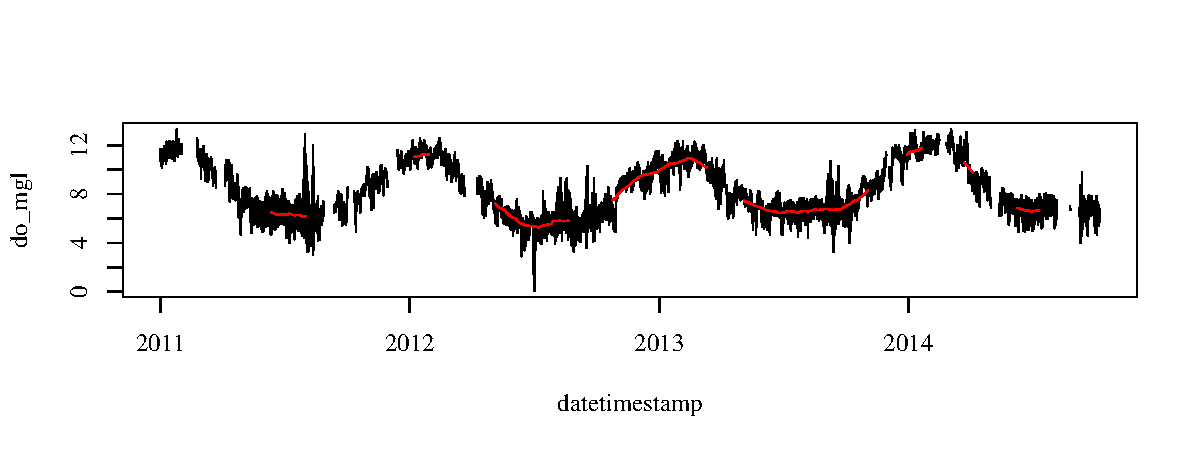
\includegraphics[width=\textwidth]{figure/unnamed-chunk-18} 

}



\end{knitrout}
\end{frame}

%%%%%%
\begin{frame}[containsverbatim]{Analysis 3 - Basic trend analysis}
This can be repeated for different time steps...
\begin{knitrout}\scriptsize
\definecolor{shadecolor}{rgb}{0.969, 0.969, 0.969}\color{fgcolor}\begin{kframe}
\begin{alltt}
\hlcom{# by season}
\hlstd{agg_dat} \hlkwb{<-} \hlkwd{aggregate}\hlstd{(dat,} \hlkwc{by} \hlstd{=} \hlstr{'quarters'}\hlstd{,} \hlkwc{params} \hlstd{=} \hlstr{'do_mgl'}\hlstd{,} \hlkwc{aggs_out} \hlstd{= T)}
\hlkwd{boxplot}\hlstd{(do_mgl} \hlopt{~} \hlstd{datetimestamp,} \hlkwc{data} \hlstd{= agg_dat,} \hlkwc{ylab} \hlstd{=} \hlstr{'do_mgl'}\hlstd{)}
\end{alltt}
\end{kframe}

{\centering 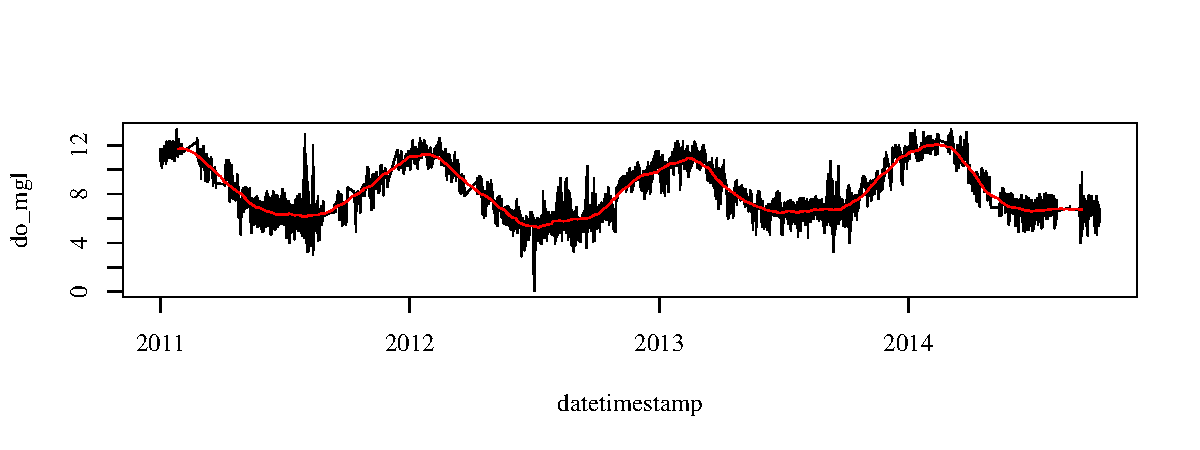
\includegraphics[width=\textwidth]{figure/unnamed-chunk-19} 

}



\end{knitrout}
\end{frame}

%%%%%%
\begin{frame}[containsverbatim]{Analysis 3 - Basic trend analysis}
This can be repeated for different time steps...
\begin{knitrout}\scriptsize
\definecolor{shadecolor}{rgb}{0.969, 0.969, 0.969}\color{fgcolor}\begin{kframe}
\begin{alltt}
\hlcom{# by year}
\hlstd{agg_dat} \hlkwb{<-} \hlkwd{aggregate}\hlstd{(dat,} \hlkwc{by} \hlstd{=} \hlstr{'years'}\hlstd{,} \hlkwc{params} \hlstd{=} \hlstr{'do_mgl'}\hlstd{,} \hlkwc{aggs_out} \hlstd{= T)}
\hlkwd{boxplot}\hlstd{(do_mgl} \hlopt{~} \hlstd{datetimestamp,} \hlkwc{data} \hlstd{= agg_dat,} \hlkwc{ylab} \hlstd{=} \hlstr{'do_mgl'}\hlstd{)}
\end{alltt}
\end{kframe}

{\centering 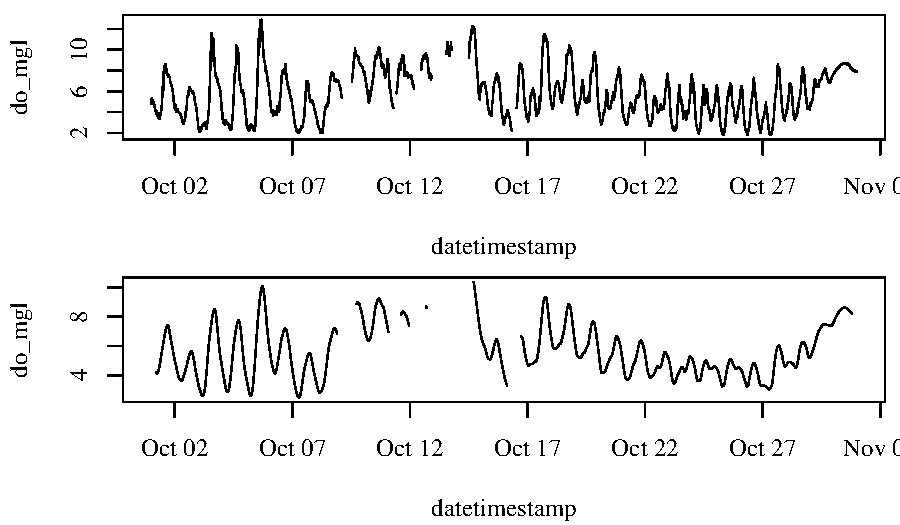
\includegraphics[width=\textwidth]{figure/unnamed-chunk-20} 

}



\end{knitrout}
\end{frame}

%%%%%%
\begin{frame}{Analysis 3 - Basic trend analysis}
A final note about trend analysis -- this can be as simple or as complex as you like \\~\\
The key question - has my variable of interest significantly changed and when did it occur? \\~\\
You must define what change means and how you will assess \\~\\
E.g., Has it increased/decreased?  How has the central tendency changed?  Has the variance changed?  What factors could have influenced this change?  \\~\\
As a first step, always plot the raw or summarized data! \\~\\
More detailed approaches are beyond the scope of this workshop - but check out the CRAN task view on \href{http://cran.r-project.org/web/views/TimeSeries.html}{time series} for more you can do in R!
\end{frame}

%%%%%%
\begin{frame}
\vspace{0.3in}
\centerline{
\begin{tikzpicture}
  \node[drop shadow={shadow xshift=0ex,shadow yshift=0ex},fill=white,draw] at (0,0) {
\includegraphics[width=0.9\textwidth]{bg_main.jpg}};
\end{tikzpicture}}
\vspace{0.5in}
\Large
\centerline{\Bigtxt{Questions??}}
\end{frame}

\end{document}
